\section{Fisica della Tomografia ad Emissione di Positroni}
Il principio alla base delle tecniche PET consiste nella rilevazione simultanea di due raggi \textGamma generati da un evento di annichilazione \textit{elettrone-positrone}, generato da iniezione di un tracciante radioattivo in un soggetto. I positroni sono emessi dal nucleo di isotopi instabili e ricchi di protoni, durante il processo di decadimento radioattivo \cite{Bailey2014}. Infatti, questi isotopi acquisiscono la stabilità tramite un processo di decadimento che converte un protone in un neutrone, con la generazione di un positrone. Il positrone, chiamato anche \textit{antielettrone}, è l'antiparticella dell'elettrone. Infatti, esso ha la stessa massa e spin 1/2 dell'elettrone ma presenta una carica elettrica \textit{+e}. Più precisamente, il processo di decadimento che si verifica è di tipo \textit{beta plus} ($\beta^+$) in cui un protone legato ($p$) del nucleo dell'isotopo radioattivo si trasforma in un neutrone legato, un positrone ($e^+$) e un neutrino ($\nu_e$) \cite{Betaplus}. Il processo può essere riassunto dalla equazione:
\begin{equation}
	\text{p}\to \text{n} + e^+ + \nu_e.
\end{equation}
I \textit{tracer} radioattivi utilizzati nelle applicazione PET sono analoghi delle comuni molecole biologiche, come il glucosio, peptidi e proteine, in cui l'isotopo radioattivo viene utilizzato per sostituire un costituente della molecola. Un radiotracciante utilizzato per la tomografia ad emissione di positroni è il fluorodeossiglucosio (FDG), un analogo strutturale del glucosio, che viene captato dalle cellule ad alto utilizzo di glucosio, come quelle del cervello, del rene e quelle tumorali \cite{FDG}. Questa molecola è soggetta al decadimento, che porta la seguente reazione:
\begin{equation}
	^{18}_9\text{F}\to ^{18}_8\text{O} + e^+ + \nu_e.
\end{equation}
La molecola risultante diviene quindi una vera e propria molecola di \textit{glucosio-6-fosfato} normalmente metabolizzata dall'organismo. Per questa ragione, questa molecola può essere utilizzata per valutare la biodistribuzione del glucosio nell'organismo.

Una volta che il \textit{tracer} radioattivo è stato iniettato al paziente, raggiunge i tessuti target grazie al sistema circolatorio e dopo un certo tempo partecipa ai processi metabolici del soggetto. Durante il decadimento del tracciatore (circa 110 minuti per il $^{18}_9\text{F}$), i positroni generati collidono con gli elettroni degli atomi adiacenti tramite un processo di \textit{annichilazione positrone-elettrone} (\Fig\ref{fig:annihilation}). L'annichilazione genera due raggi gamma con un energia di \SI{511}{\kilo\electronvolt}, con un angolazione di circa \SI{180}{\degree}.
\begin{figure}[h]
	\centering
	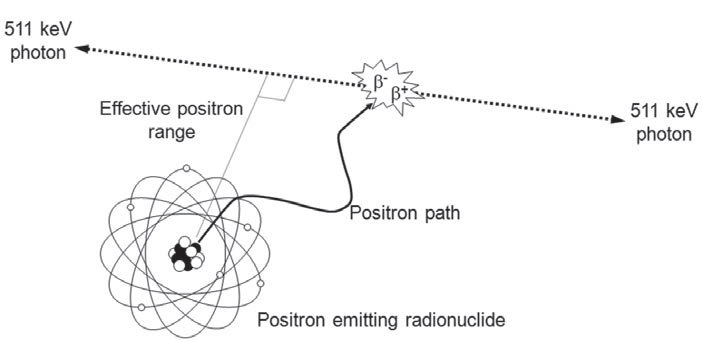
\includegraphics[width=0.8\linewidth]{./ImageFiles/annihilation}
	\caption{Processo di annichilazione \textit{positrone-elettrone} con generazione di due raggi gamma. Immagine tratta da Bailey D. et al\cite{Bailey2014}.}
	\label{fig:annihilation}
\end{figure}

\section{Sistema PET}
Nella figura \ref{fig:PET_imaging_system} è rappresentato un sistema di imaging PET. 
\begin{figure}[h]
	\centering
	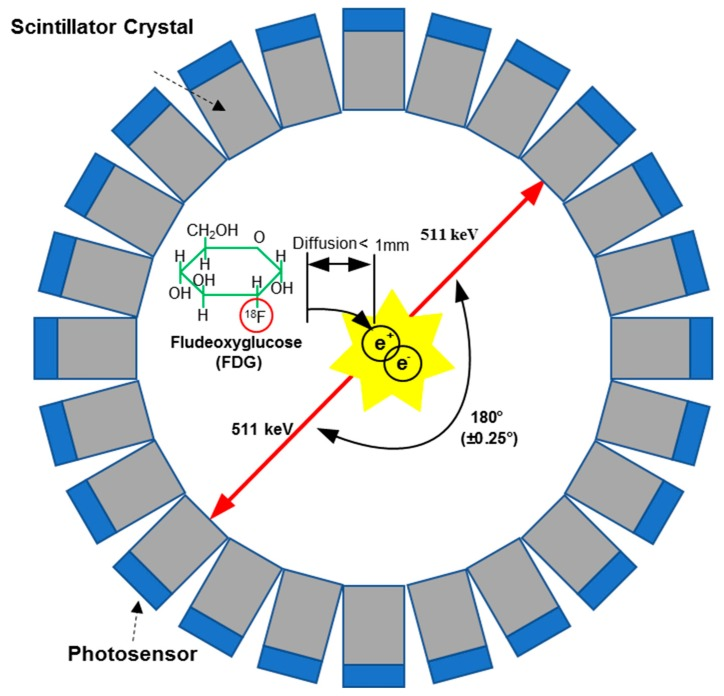
\includegraphics[width=0.8\linewidth]{./ImageFiles/PET_imaging_system}
	\caption{Principio di funzionamento di un sistema per tomografia ad emissione di positroni (PET). Un anello di sensori rilevano una coppia di raggi gamma con un'energia di \SI{511}{3\kilo\electronvolt} (frecce rosse) che derivano dalla annichilazione di un elettrone con un positrone emesso da un radiotracciante (FDG). Immagine tratta da Jiang W. et al \cite{Jiang2019}.}
	\label{fig:PET_imaging_system}
\end{figure}
Per rilevare i raggi gamma derivanti dal processo di annichilazione \textit{elettrone-positrone}, viene utilizzato un rilevatore a scintillazione, composto da uno scintillatore e un fotorilevatore. I cristalli scintillatori sono utilizzati per assorbire e convertire un raggio gamma ad alta energia in fotoni visibili a bassa energia, rilevati da opportuni sensori. Uno dei cristalli scintillatori più utilizzati è il \textit{Lutetium–(yttrium) oxyorthosilicate} (L(Y)SO) che garantisce una buona risoluzione di energia, alta luminosità in uscita e un tempo veloce di decadimento. Il processo di conversione di fotoni ad alta energia (raggi \textgamma) in luce visibile consiste in tre fasi \cite{RamseyDerek}:
\begin{itemize}
	\item un fotone incidente sul cristallo libera un elettrone (tramite effetto fotoelettrico o effetto Compton);
	\item quando l'elettrone attraversa il materiale, perde energia urtando ed eccitando altri elettroni;
	\item gli elettroni eccitati ritornano decadono al loro stato base, emettendo fotoni (sotto forma di impulsi di luce nel visibile).
\end{itemize}
Gli scintillatori utilizzati nei sistemi di acquisizione PET possono essere differenziati considerando quattro diverse proprietà \cite{Schmitz2013ThePO}:
\begin{itemize}
	\item stopping power;
	\item decay constant;
	\item energy resolution;
	\item light output.
\end{itemize}
Lo \textbf{stopping power} rappresenta l'inverso della distanza media percorsa dai fotoni prima di trasferire l'energia nel cristallo e dipende dalla densità e dal numero atomico effettivo del materiale. \`E preferibile che questo parametro sia alto (ossia poca distanza percorsa dai fotoni), in modo da avere più interazioni con i fotoni emessi dall'annichilazione \textit{elettrone-positrone}. La \textbf{decay constant}, invece, descrive la durata dell'impulso luminoso generato dal cristallo. \`E preferibile utilizzare cristalli con bassi valori di constante di decadimento in quanto permettono di rilevare un numero maggiore di impulsi a pari unità di tempo. Inoltre, è utile che il materiale abbia una buona risoluzione di energia (\textbf{energy resolution}), che descrive la capacità di distinguere raggi gamma con differenti energie. Infatti, nell'immagine \ref{fig:photo_peak} è mostrato lo spettro di distribuzione di energia, costruito misurando il numero di eventi rilevati con una certa ampiezza in funzione dell'energia depositata sul cristallo.
\begin{figure}[h]
	\centering
	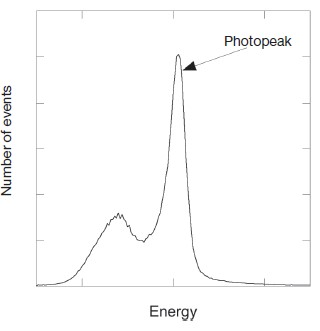
\includegraphics[width=0.8\linewidth]{./ImageFiles/Photo peak.jpg}
	\caption{Esempio di uno spettro di energia, definito come il numero di eventi misurati con una certa ampiezza in funzione della energia depositata sul cristallo. Immagine tratta da Bailey D et al. \cite{Bailey2014}.}
	\label{fig:photo_peak}
\end{figure}
Questa distribuzione è influenzata dalle caratteristiche del tracciatore radioattivo utilizzato e dal materiale con cui è realizzato il rilevatore. Tuttavia, è possibile sempre notare un picco marcato (denominato \textit{photopeak}), causato dall'assorbimento fotoelettrico, dove tutta l'energia del fotone è trasmessa all'elettrone. L'altra regione in cui l'energia si distribuisce è invece causata dall'effetto Compton, dove gli elettroni acquistano diversi valori di energia in base all'angolo di scattering.